% Options for packages loaded elsewhere
\PassOptionsToPackage{unicode}{hyperref}
\PassOptionsToPackage{hyphens}{url}
\documentclass[
]{article}
\usepackage{xcolor}
\usepackage[margin=1in]{geometry}
\usepackage{amsmath,amssymb}
\setcounter{secnumdepth}{-\maxdimen} % remove section numbering
\usepackage{iftex}
\ifPDFTeX
  \usepackage[T1]{fontenc}
  \usepackage[utf8]{inputenc}
  \usepackage{textcomp} % provide euro and other symbols
\else % if luatex or xetex
  \usepackage{unicode-math} % this also loads fontspec
  \defaultfontfeatures{Scale=MatchLowercase}
  \defaultfontfeatures[\rmfamily]{Ligatures=TeX,Scale=1}
\fi
\usepackage{lmodern}
\ifPDFTeX\else
  % xetex/luatex font selection
\fi
% Use upquote if available, for straight quotes in verbatim environments
\IfFileExists{upquote.sty}{\usepackage{upquote}}{}
\IfFileExists{microtype.sty}{% use microtype if available
  \usepackage[]{microtype}
  \UseMicrotypeSet[protrusion]{basicmath} % disable protrusion for tt fonts
}{}
\makeatletter
\@ifundefined{KOMAClassName}{% if non-KOMA class
  \IfFileExists{parskip.sty}{%
    \usepackage{parskip}
  }{% else
    \setlength{\parindent}{0pt}
    \setlength{\parskip}{6pt plus 2pt minus 1pt}}
}{% if KOMA class
  \KOMAoptions{parskip=half}}
\makeatother
\usepackage{longtable,booktabs,array}
\newcounter{none} % for unnumbered tables
\usepackage{calc} % for calculating minipage widths
% Correct order of tables after \paragraph or \subparagraph
\usepackage{etoolbox}
\makeatletter
\patchcmd\longtable{\par}{\if@noskipsec\mbox{}\fi\par}{}{}
\makeatother
% Allow footnotes in longtable head/foot
\IfFileExists{footnotehyper.sty}{\usepackage{footnotehyper}}{\usepackage{footnote}}
\makesavenoteenv{longtable}
\usepackage{graphicx}
\makeatletter
\newsavebox\pandoc@box
\newcommand*\pandocbounded[1]{% scales image to fit in text height/width
  \sbox\pandoc@box{#1}%
  \Gscale@div\@tempa{\textheight}{\dimexpr\ht\pandoc@box+\dp\pandoc@box\relax}%
  \Gscale@div\@tempb{\linewidth}{\wd\pandoc@box}%
  \ifdim\@tempb\p@<\@tempa\p@\let\@tempa\@tempb\fi% select the smaller of both
  \ifdim\@tempa\p@<\p@\scalebox{\@tempa}{\usebox\pandoc@box}%
  \else\usebox{\pandoc@box}%
  \fi%
}
% Set default figure placement to htbp
\def\fps@figure{htbp}
\makeatother
\setlength{\emergencystretch}{3em} % prevent overfull lines
\providecommand{\tightlist}{%
  \setlength{\itemsep}{0pt}\setlength{\parskip}{0pt}}
% Override Pandoc's \pandocbounded (fits image to BOTH \linewidth and \textheight).
% That shrinks tall multi-panel PNGs much more than Markdown/HTML preview, which
% typically scales by width only. Scale to line width; allow tall figures to use
% vertical space (may span pages).
\usepackage{float}
\floatplacement{figure}{H}

\makeatletter
\renewcommand*\pandocbounded[1]{%
  \sbox\pandoc@box{#1}%
  \Gscale@div\@tempa{\linewidth}{\wd\pandoc@box}%
  \ifdim\@tempa\p@<\p@\scalebox{\@tempa}{\usebox\pandoc@box}%
  \else\usebox{\pandoc@box}%
  \fi%
}
\makeatother
\usepackage{bookmark}
\IfFileExists{xurl.sty}{\usepackage{xurl}}{} % add URL line breaks if available
\urlstyle{same}
\hypersetup{
  hidelinks,
  pdfcreator={LaTeX via pandoc}}

\author{}
\date{}

\begin{document}

\section{Exploratory Data Analysis: Singapore Total Live Births and
Total Fertility Rate
(1960--2024)}\label{exploratory-data-analysis-singapore-total-live-births-and-total-fertility-rate-19602024}

\textbf{Author:} Minh Chien Nguyen\\
\textbf{GitHub Repository:}
\url{https://github.com/perryx05/Time-Series-Analysis}

\begin{center}\rule{0.5\linewidth}{0.5pt}\end{center}

\subsection{1. Introduction and Research
Questions}\label{introduction-and-research-questions}

Singapore has experienced a significant demographic transition since
gaining independence, going from a high-fertility country in the 1960s
to having one of the lowest fertility rates in the world by the 2000s.
Understanding the trends in Total Live Births (TLB) and Total Fertility
Rate (TFR) is important for demographic forecasting and policy
evaluation.

This EDA investigates the following research questions:

\begin{enumerate}
\def\labelenumi{\arabic{enumi}.}
\tightlist
\item
  \textbf{What are the key temporal trends and structural changes in
  Singapore's TLB and TFR from 1960 to 2024?}
\item
  \textbf{Which possible time series models are appropriate for
  forecasting TLB and TFR beyond the training period (1960--2012)?}
\item
  \textbf{To what extent do known social and policy events explain the
  observed patterns in TLB and TFR?}
\end{enumerate}

\begin{center}\rule{0.5\linewidth}{0.5pt}\end{center}

\subsection{2. Data Description}\label{data-description}

\textbf{Source:} Singapore Department of Statistics (singstat.gov.sg)\\
\textbf{Variables of interest:}

\begin{itemize}
\tightlist
\item
  \textbf{Total Live Births (TLB):} Annual count of live births in
  Singapore
\item
  \textbf{Total Fertility Rate (TFR):} Average number of children a
  woman would have over her lifetime, based on current age-specific
  fertility rates
\end{itemize}

\textbf{Period:} 1960 to 2024 (65 annual observations)\\
\textbf{Frequency:} Annual (no seasonality)\\
\textbf{Split:} Training set 1960--2012 (53 observations); test set
2013--2024 (12 observations)

\subsubsection{2.1 Data Limitations}\label{data-limitations}

\begin{itemize}
\tightlist
\item
  Annual aggregation cannot highlight the intra-year variation.
\item
  TFR is a period measure and does not directly reflect completed
  fertility of any cohort.
\item
  \textbf{Coverage definition (SingStat):} TFR before 1980 refers to the
  \textbf{total population}; from 1980 onward it refers to the
  \textbf{resident population} (citizens and permanent residents).
  Long-run comparisons should consider this change.
\item
  Policy interventions and external shocks (e.g., economic recessions,
  COVID-19) create structural breaks that standard time series models
  may not capture well.
\item
  No missing values were identified in the dataset.
\end{itemize}

\begin{center}\rule{0.5\linewidth}{0.5pt}\end{center}

\subsection{3. Data Cleaning}\label{data-cleaning}

The raw data was downloaded from singstat.gov.sg and saved as a CSV
file. The following cleaning steps were applied:

\begin{enumerate}
\def\labelenumi{\arabic{enumi}.}
\tightlist
\item
  Extracted only the two required series from the SingStat wide-format
  export: \texttt{Total\ Live-Births\ (Number)} and
  \texttt{Total\ Fertility\ Rate\ (TFR)\ (Per\ Female)}.
\item
  Reshaped from wide year-columns format into a tidy table with only 3
  columns \texttt{Year}, \texttt{TLB}, \texttt{TFR}.
\item
  Removed comma formatting from TLB values and converted both series to
  numeric.
\item
  Verified no missing values were present in either series.
\item
  Confirmed 65 rows and plausible value ranges:

  \begin{itemize}
  \tightlist
  \item
    TLB: 33,541 to 61,775
  \item
    TFR: 0.97 to 5.76
  \end{itemize}
\item
  Saved cleaned data as \texttt{cleaned\_tlb\_tfr\_1960\_2024.csv} for
  use in later sections.
\item
  Created annual time series objects (\texttt{tlb\_ts},
  \texttt{tfr\_ts}) and the required training/test splits:

  \begin{itemize}
  \tightlist
  \item
    Training: 1960--2012
  \item
    Test: 2013--2024
  \end{itemize}
\end{enumerate}

\begin{center}\rule{0.5\linewidth}{0.5pt}\end{center}

\subsection{4. Visualisation and Temporal
Features}\label{visualisation-and-temporal-features}

\subsubsection{4.1 Overview panel}\label{overview-panel}

\begin{figure}
\centering
\pandocbounded{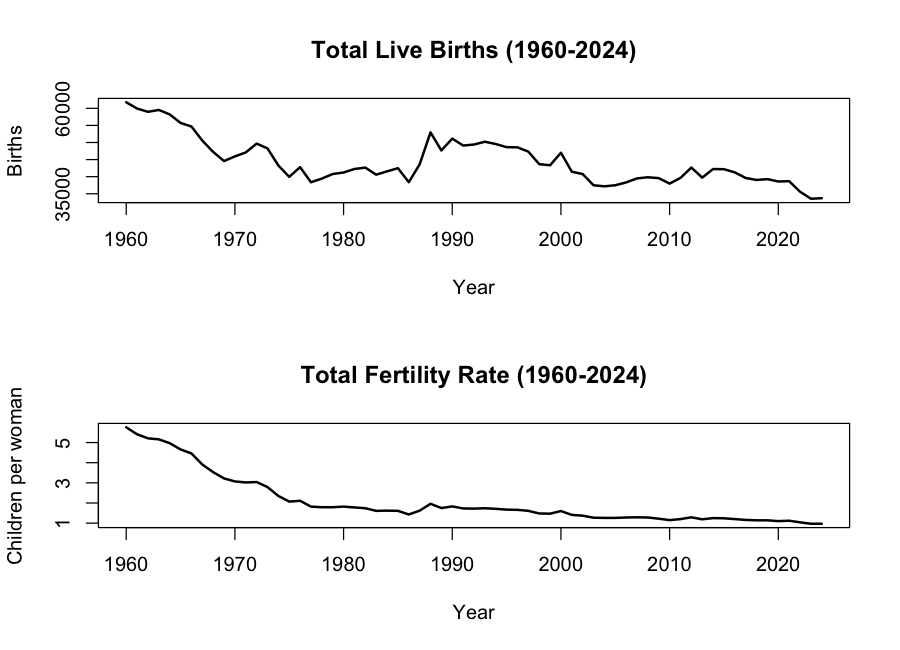
\includegraphics[keepaspectratio,alt={TLB and TFR overview (1960--2024)}]{plots/00_overview_panel.png}}
\caption{TLB and TFR overview (1960--2024)}
\end{figure}

Looking at the two graphs together we can have a good starting point for
understanding the data. The Total Live Births (TLB) number tends to move
up and down quite a lot from year to year. It drops quite sharply from
the early 1960s, then there is a noticeable increase around the late
1980s, and after the 2000s it stays at a generally lower level. There is
also a clear fall happening around 2020 to 2022. For the Total Fertility
Rate (TFR), the overall pattern looks similar, but the line is much
smoother compared to TLB. This makes sense because TFR is calculated
from age-specific birth rates, so it does not get affected by the total
population size in the same way as the raw birth count does. Since this
data is recorded every year, there is no seasonal pattern to observe.
The main thing we can see is the long-term downward trend, with some
short periods where the numbers went slightly higher or lower than
expected.

\subsubsection{4.2 Total Live Births
(1960--2024)}\label{total-live-births-19602024}

\begin{figure}
\centering
\pandocbounded{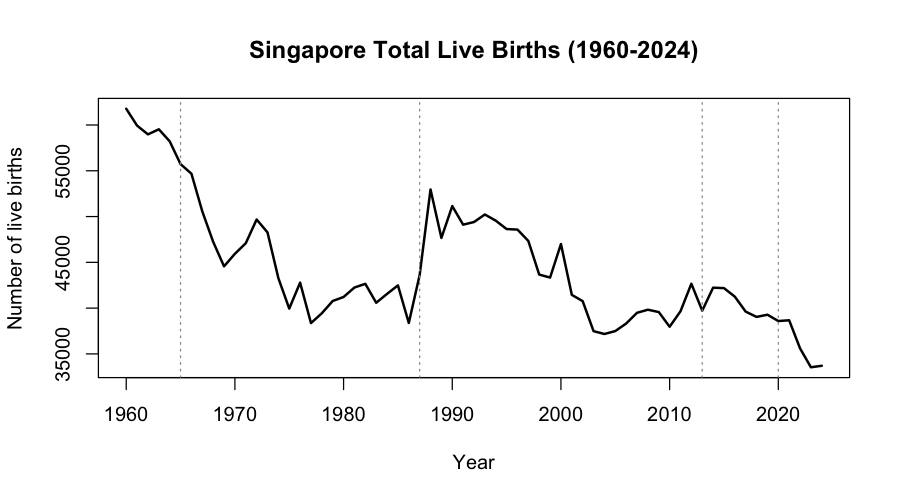
\includegraphics[keepaspectratio,alt={Singapore Total Live Births, 1960--2024}]{plots/01_tlb_full.png}}
\caption{Singapore Total Live Births, 1960--2024}
\end{figure}

\begin{itemize}
\tightlist
\item
  \textbf{Early 1960s:} TLB was high (about 61,000 in 1960), but then it
  dropped quite sharply through the late 1960s and 1970s. This may be
  connected to intensive government policy and social change to reduce
  births after independence. For example, the Singapore Family Planning
  and Population Board was established in 1966 as part of a national
  programme to control population growth (OBGyn Key n.d.).
\item
  \textbf{Late 1980s:} The number of births increased slightly, which
  could be related to the change in government message at that time.
  Specifically, the \textbf{``Have Three or More if You Can Afford It''}
  campaign was announced in 1987 (National Library Board Singapore
  2000). But this increase did not last long and the number did not go
  back to the same level as the 1960s.
\item
  \textbf{1990s--2010s:} Births continued to slowly go down, but with
  some up and down movement along the way. This is likely due to several
  reasons happening at the same time --- such as people getting married
  later, more women working, and the high cost of housing and childcare
  --- rather than one simple cause.
\item
  \textbf{From 2013:} The dotted vertical line around 2013 marks the
  beginning of the period used to test how well the forecasting model
  performs, which covers 2013 to 2024. The birth numbers remain quite
  low; 2020 is marked as a year when external shocks (COVID-19) may have
  affected when babies were born and when births were officially
  recorded.
\end{itemize}

For time series modelling, the figure suggests that treating TLB as
\textbf{non-stationary} (clear level shift and trend) rather than
fluctuating around a fixed mean.

\subsubsection{4.3 Total Fertility Rate
(1960--2024)}\label{total-fertility-rate-19602024}

\begin{figure}
\centering
\pandocbounded{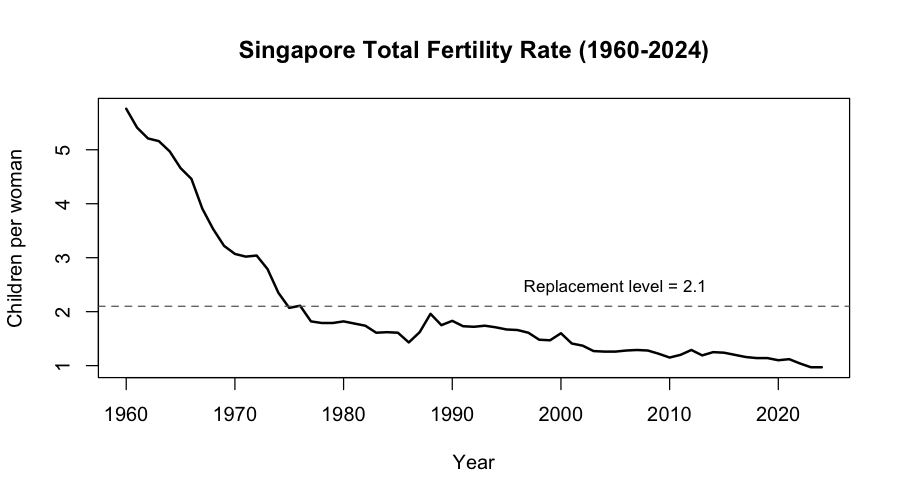
\includegraphics[keepaspectratio,alt={Singapore Total Fertility Rate, 1960--2024}]{plots/02_tfr_full.png}}
\caption{Singapore Total Fertility Rate, 1960--2024}
\end{figure}

TFR starts near \textbf{5.8} in 1960 and drops below \textbf{2} by the
mid-1970s. The horizontal dashed line at \textbf{2.1} is
\textbf{replacement-level fertility} (a standard demographic benchmark;
see United Nations Statistics Division n.d.). Singapore's TFR has
remained below that line for many decades, reaching roughly \textbf{1.0}
in recent years, which is considered extremely low and is a major
concern for the government when thinking about whether the population
can replace itself naturally.

Because SingStat notes a \textbf{change in population coverage} for TFR
in \textbf{1980} (total population before 1980; resident population from
1980 onward), the level around 1979--1981 should be interpreted
cautiously when arguing about precise ``breaks''. However, this
technical detail does not really change the overall picture --- it is
still very clear from the graph that Singapore's fertility rate
collapsed dramatically over this period.

\subsubsection{4.4 TLB and TFR on one figure (dual vertical
axis)}\label{tlb-and-tfr-on-one-figure-dual-vertical-axis}

\begin{figure}
\centering
\pandocbounded{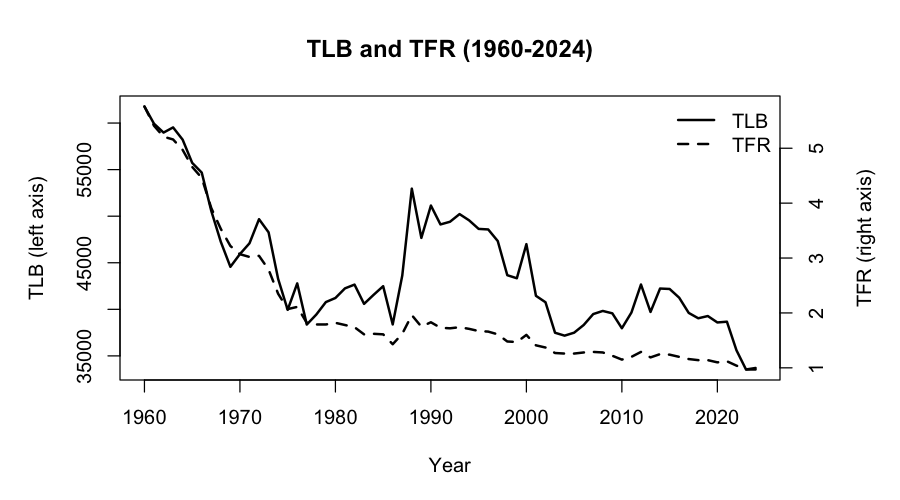
\includegraphics[keepaspectratio,alt={TLB and TFR combined, 1960--2024}]{plots/03_tlb_tfr_combined.png}}
\caption{TLB and TFR combined, 1960--2024}
\end{figure}

This plot is not for reading exact numbers between two measurements
(births vs.~rate). It is useful to see \textbf{how the two lines move
together over time}: both series decline together in the first two
decades; both show a small increase in the \textbf{late 1980}; both end
up at low levels in the \textbf{2000s and 2010s}. However, there are
some short periods where the total live births line moves more sharply
up or down compared to the TFR line. This can happen because TLB is also
affected by things like how many women of childbearing age are in the
population at a given time, or changes due to migration --- not just
whether women are choosing to have more or fewer children. This is one
of the reasons why it makes more sense to model TLB and TFR as two
separate series, rather than assuming that one is simply a scaled-up or
scaled-down version of the other.

\subsubsection{4.5 Training vs test split (modelling
design)}\label{training-vs-test-split-modelling-design}

\begin{figure}
\centering
\pandocbounded{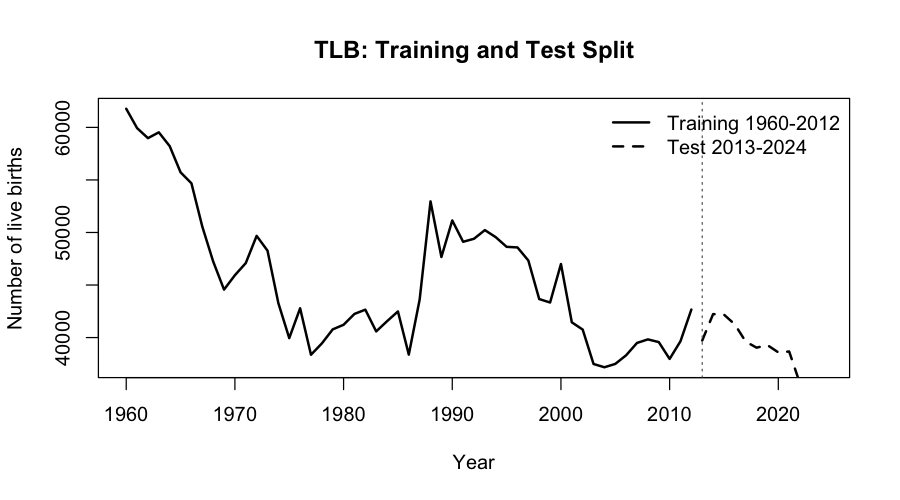
\includegraphics[keepaspectratio,alt={TLB: training vs test}]{plots/04_tlb_train_test_split.png}}
\caption{TLB: training vs test}
\end{figure}

\begin{figure}
\centering
\pandocbounded{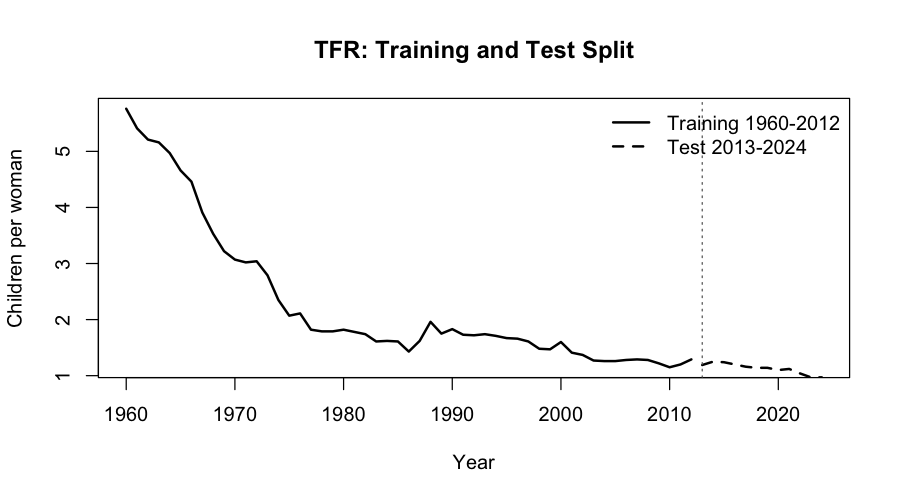
\includegraphics[keepaspectratio,alt={TFR: training vs test}]{plots/05_tfr_train_test_split.png}}
\caption{TFR: training vs test}
\end{figure}

The data is divided into two parts. The first part, from \textbf{1960 to
2012 (53 years)}, is used to train the models, while the second part,
from \textbf{2013 to 2024 (12 years)}, is used to test how good the
models can forecast. In each graph, the solid line represents the
training period and the dashed line represents the test period, with a
vertical marker showing where the split happens at 2013.

For the \textbf{Total Live Births}, the training period covers the most
significant drops in birth numbers as well as the small increase in the
late 1980s. The test period, on the other hand, includes the fall in
births that happened around the COVID-19 period and some recovery
afterwards. For the Total Fertility Rate, the test period stays within a
quite narrow and very low range of roughly 1.0 to 1.3 children per
woman. This means the models, which were only trained on data before
2013, need to make predictions for a period where fertility is already
extremely low --- quite far from where it started in the 1960s.

\subsubsection{\texorpdfstring{4.6 Trend smoothing and what we do
\emph{not} use (STL / seasonal
decomposition)}{4.6 Trend smoothing and what we do not use (STL / seasonal decomposition)}}\label{trend-smoothing-and-what-we-do-not-use-stl-seasonal-decomposition}

For annual data there is no seasonal period within the year:
\texttt{frequency\ =\ 1}, so STL decomposition and classical seasonal
decomposition are not appropriate --- they require a seasonal cycle
(e.g.~monthly s=12, quarterly s=4).

Our approach uses a \textbf{centred moving average} to approximate a
\textbf{smooth trend}; what is left over when comparing the annual
series to that trend is informal irregular variation.

\begin{figure}
\centering
\pandocbounded{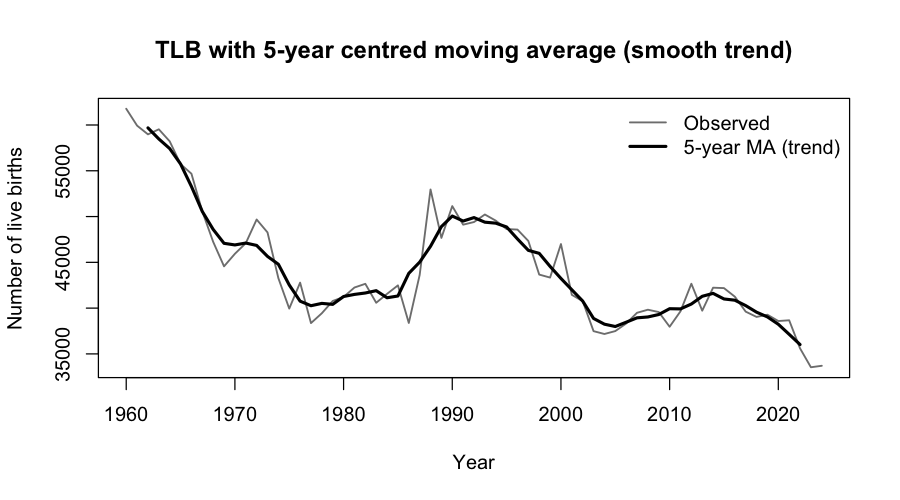
\includegraphics[keepaspectratio,alt={TLB with 5-year centred MA}]{plots/06_tlb_ma_trend.png}}
\caption{TLB with 5-year centred MA}
\end{figure}

\begin{figure}
\centering
\pandocbounded{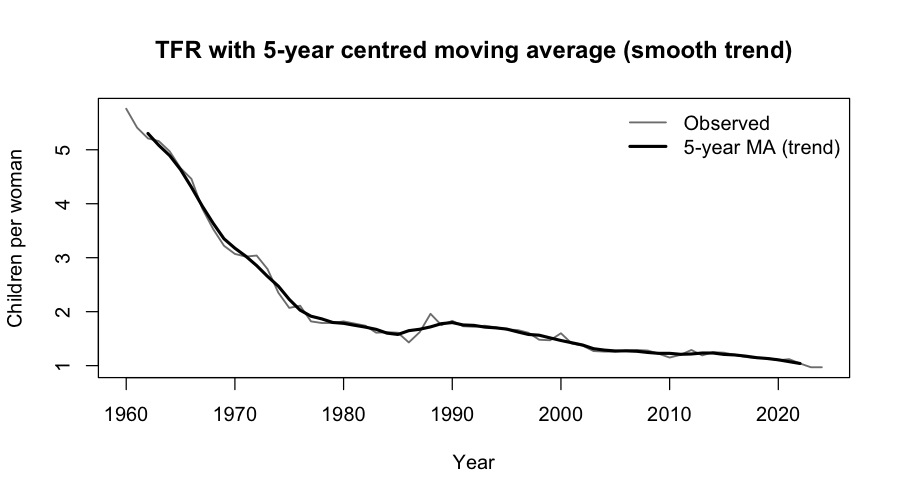
\includegraphics[keepaspectratio,alt={TFR with 5-year centred MA}]{plots/07_tfr_ma_trend.png}}
\caption{TFR with 5-year centred MA}
\end{figure}

\textbf{Why a 5-year window.} A 5-year centred moving average was
selected over shorter or longer windows. A 3-year MA retains too much of
the short-term ups and downs in the data, while a 7-year MA over-smooths
and ends up hiding some important changes in the mid-1970s and late
1980s. The 5-year window also aligns with Singapore's governmental
planning cycles, providing a substantively meaningful smoothing
interval. Another practical reason for using a 5-year odd-ordered
centred moving average is that it does not require an extra re-centring
step, which would be needed if an even-numbered window was used instead.

\begin{center}\rule{0.5\linewidth}{0.5pt}\end{center}

\subsection{5. Social and Economic
Context}\label{social-and-economic-context}

The patterns visible in TLB and TFR cannot be fully understood through
statistical analysis. Several known policy events and social changes
have directly shaped the data, and any time series model trained on this
period will be implicitly fitting through these structural changes.

\begin{itemize}
\tightlist
\item
  \textbf{1966 --- Family planning campaign:} The Singapore Family
  Planning and Population Board was established, launching an active
  campaign to discourage large families. This is closely associated with
  the sharp decline in TLB and TFR through the late 1960s and 1970s
  (OBGyn Key n.d.).
\item
  \textbf{1987 --- "Have Three or More" policy:} The government reversed
  its earlier position and introduced a pro-natalist message encouraging
  Singaporeans to have three or more children if they could afford it
  (National Library Board Singapore 2000). An increase in births is
  visible around this period, but the effect was temporary and small
  relative to the long-run decline.
\item
  \textbf{1990s--2000s --- Baby Bonus and other incentives:} The
  government introduced a range of financial supports, childcare
  subsidies, and housing priority policies to support families. Despite
  these efforts, TFR continued to fall, suggesting that many economic
  factors --- high cost of living, delayed marriage, female labour force
  participation --- were more dominant than policy supports alone.
\item
  \textbf{2020--2021 --- COVID-19:} The pandemic disrupted family
  formation patterns globally. A visible decrease in TLB around
  2020--2021 is consistent with international trends where economic
  uncertainty and lockdown conditions led couples to postpone having
  children.
\end{itemize}

These events are important for model selection in the Final Report. A
purely statistical model may not adequately capture these discrete
structural changes, and any model that performs poorly on the 2013--2024
test period should be evaluated in light of whether the test period
itself was unusual by historical standards (for example, COVID-19).

\begin{center}\rule{0.5\linewidth}{0.5pt}\end{center}

\subsection{6. Analysis of Time Series
Features}\label{analysis-of-time-series-features}

Following the workflow, all analytics in this section use
\textbf{training data only (1960--2012)}: \textbf{raw} ACF/PACF, then
\textbf{first differences} (annual change---each year minus the year
before), then ACF/PACF of the differenced series. This is exploratory
description of autocorrelation only.

\subsubsection{6.1 ACF and PACF (raw) and first
differences}\label{acf-and-pacf-raw-and-first-differences}

\textbf{Raw series}

\begin{figure}
\centering
\pandocbounded{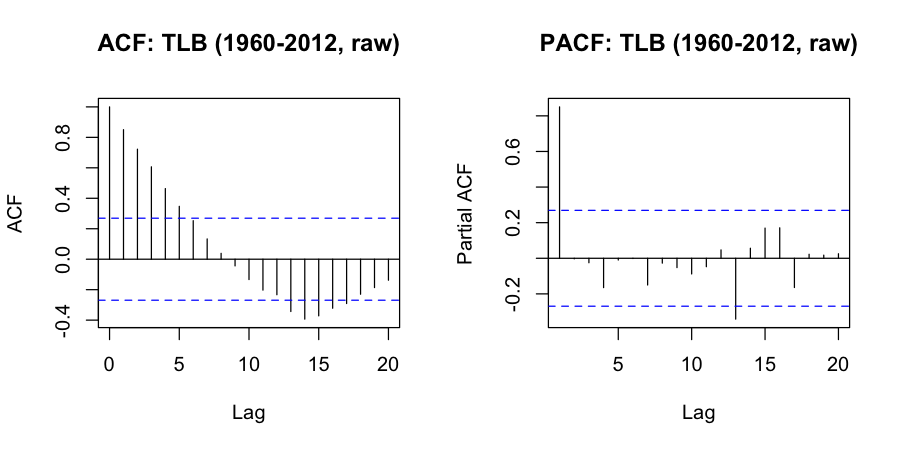
\includegraphics[keepaspectratio,alt={ACF/PACF TLB raw}]{plots/08_tlb_acf_pacf_raw.png}}
\caption{ACF/PACF TLB raw}
\end{figure}

\begin{figure}
\centering
\pandocbounded{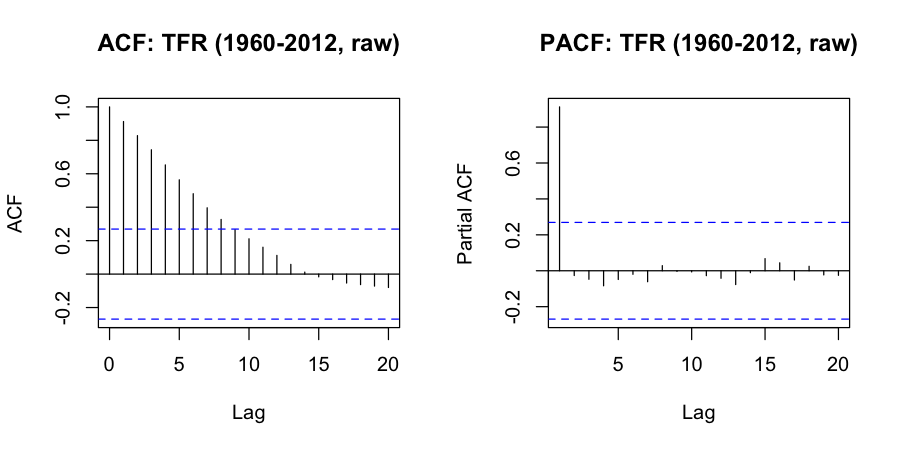
\includegraphics[keepaspectratio,alt={ACF/PACF TFR raw}]{plots/09_tfr_acf_pacf_raw.png}}
\caption{ACF/PACF TFR raw}
\end{figure}

For both \textbf{TLB} and \textbf{TFR} \textbf{ACF} plot, the bars stay
quite high and drop down very slowly across many lags. This kind of
pattern usually means the data has a strong memory --- values from many
years ago are still closely related to values today. This is a clear
sign that both series are non-stationary, meaning they do not fluctuate
around a fixed average but instead follow a long-running downward trend
over time, which is consistent with what is sometimes called unit-root
or near unit-root behaviour. The PACF patterns are not the useful tool
until after differencing; trying to read it as a simple low-order
autoregressive pattern on the original untransformed data would not give
a meaningful or reliable result.

\textbf{First differences (illustrative series)}

\begin{figure}
\centering
\pandocbounded{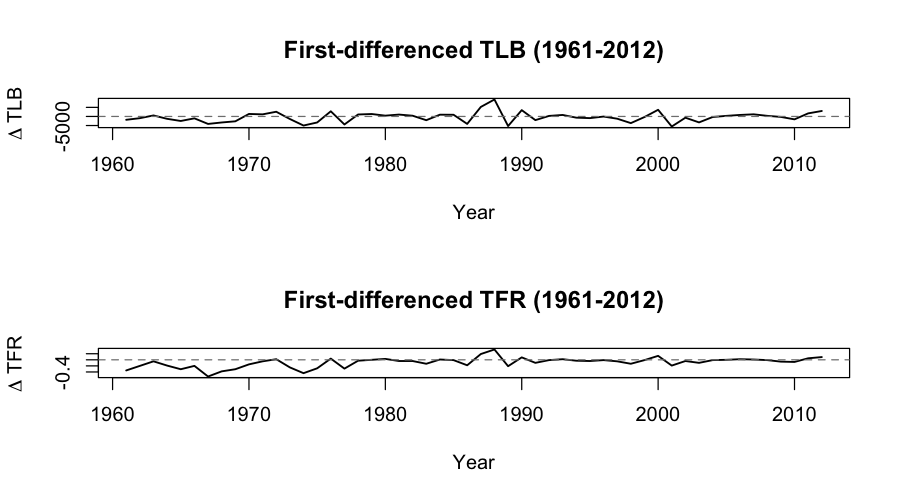
\includegraphics[keepaspectratio,alt={First-differenced TLB and TFR}]{plots/10_differenced_series.png}}
\caption{First-differenced TLB and TFR}
\end{figure}

After applying first differencing, both series now fluctuate around zero
without any clear upward or downward drift. This means the data is now
showing the year-to-year change --- how much the number of births or the
fertility rate went up or down compared to the previous year --- rather
than the overall level. This transformed version of the data is more
suitable for modelling because it captures the accumulated effect of
short-term shocks and the influence of different policy phases over
time.

\textbf{ACF/PACF after differencing}

\begin{figure}
\centering
\pandocbounded{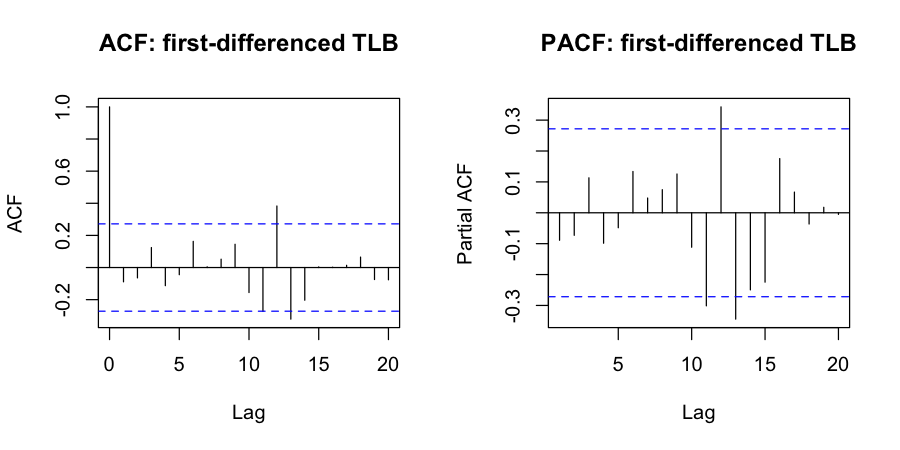
\includegraphics[keepaspectratio,alt={ACF/PACF first-differenced TLB}]{plots/11_tlb_acf_pacf_diff.png}}
\caption{ACF/PACF first-differenced TLB}
\end{figure}

\begin{figure}
\centering
\pandocbounded{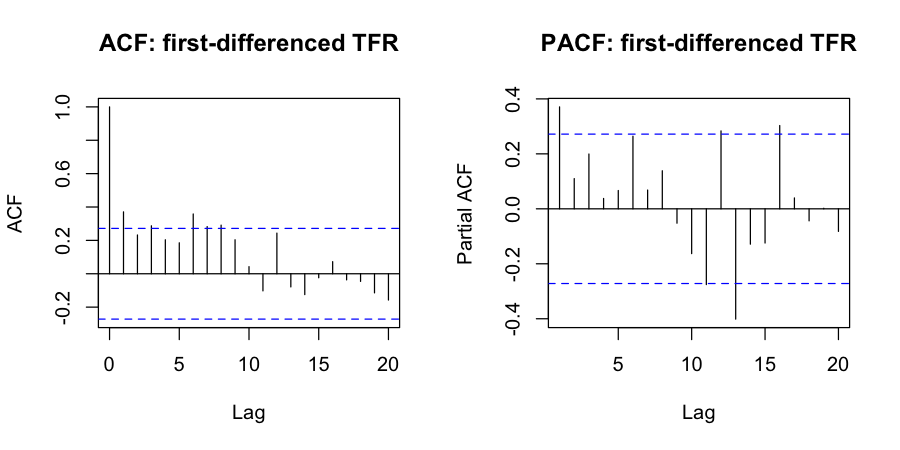
\includegraphics[keepaspectratio,alt={ACF/PACF first-differenced TFR}]{plots/12_tfr_acf_pacf_diff.png}}
\caption{ACF/PACF first-differenced TFR}
\end{figure}

After \textbf{one difference}, the correlations die off much faster
compared to the original series. This is what we want because AR / MA /
ARMA models assume the series is roughly stationary around a stable
mean.

For \textbf{TLB (annual change)}, the ACF and PACF at short lags (1--3)
are mostly inside the confidence bands. This suggests the year-to-year
change in births does not have a strong and stable autocorrelation
pattern. A reasonable and very parsimonious first candidate is
\textbf{ARMA(0,0)} for the differenced series (meaning the changes are
close to white noise plus an average drift).

For \textbf{TFR (annual change)}, the PACF shows a clear spike at lag 1
while the ACF drops quickly. This pattern is often consistent with an
\textbf{AR(1)} structure on the differenced series, so a sensible first
candidate is \textbf{AR(1)} for the annual changes in TFR. Some later
lags show spikes too, but because the sample after differencing is only
52 points and fertility has structural breaks, we start with a simple
low-order model and rely on residual checks to see if the model is
acceptable.

\subsubsection{6.2 Stationarity tests}\label{stationarity-tests}

Tests are run in \textbf{R} (\texttt{tseries} package) with default
settings. \textbf{Augmented Dickey--Fuller (ADF):} \(H_0\) =
\textbf{unit root} (non-stationary); \textbf{rejection} of \(H_0\)
(small p-value, typically compared to \(\alpha = 0.05\)) supports
\textbf{stationarity}.

\textbf{Justification of the formula used above (first difference).} In
\(\Delta y_t = y_t - y_{t-1}\), \(y_t\) means the series value in year
\(t\), \(y_{t-1}\) means the previous year value, and \(\Delta y_t\) is
the year-to-year change (annual change). We use it because the level
series has strong trend, and AR/MA/ARMA needs a more stable series.

{\def\LTcaptype{none} % do not increment counter
\begin{longtable}[]{@{}
  >{\raggedright\arraybackslash}p{(\linewidth - 4\tabcolsep) * \real{0.1667}}
  >{\raggedright\arraybackslash}p{(\linewidth - 4\tabcolsep) * \real{0.2708}}
  >{\raggedright\arraybackslash}p{(\linewidth - 4\tabcolsep) * \real{0.5625}}@{}}
\toprule\noalign{}
\begin{minipage}[b]{\linewidth}\raggedright
Series
\end{minipage} & \begin{minipage}[b]{\linewidth}\raggedright
ADF p-value
\end{minipage} & \begin{minipage}[b]{\linewidth}\raggedright
Interpretation (\(\alpha = 0.05\))
\end{minipage} \\
\midrule\noalign{}
\endhead
\bottomrule\noalign{}
\endlastfoot
TLB (raw) & 0.356 & Do not reject \(H_0\) → \textbf{no evidence against
a unit root}; level treated as \textbf{non-stationary}. \\
TFR (raw) & 0.120 & Do not reject \(H_0\) → \textbf{non-stationary}
level (not significant at 5\%). \\
TLB, first difference & 0.039 & Reject \(H_0\) → \textbf{stationary}
differenced series. \\
TFR, first difference & 0.083 & Do \textbf{not} reject \(H_0\) at 5\%
(borderline); \textbf{inconclusive}---unit root not ruled out
strongly. \\
\end{longtable}
}

\textbf{Summary.} ADF on the raw series suggests both TLB and TFR are
non-stationary in levels (they have strong trend / long memory). After
one difference (annual change, \(\Delta y_t = y_t - y_{t-1}\)),
\textbf{TLB} clearly becomes stationary by ADF at 5\%. For \textbf{TFR},
the differenced ADF result is borderline at 5\%, which is not unusual
for short annual series with policy breaks. In this EDA we still proceed
with modelling the annual changes using simple AR / MA / ARMA
candidates, and we check if residuals look like white noise.

\begin{center}\rule{0.5\linewidth}{0.5pt}\end{center}

\subsection{7. Preliminary Model Identification (training:
1960--2012)}\label{preliminary-model-identification-training-19602012}

For each candidate model below, we report: - AIC and BIC (in-sample fit
with complexity penalty) - residual ACF/PACF (should look like white
noise) - Box--Ljung test on residuals (lag 10)

\textbf{Justification of terms (AIC/BIC and Box--Ljung).}\\
- \textbf{AIC/BIC}: it can be considered as \textbf{fit − penalty}.
Smaller is better. In formula form (for reference): \textbf{AIC = −2
log(L) + 2k} and \textbf{BIC = −2 log(L) + k log(n)}, where \textbf{L}
is likelihood, \textbf{k} is number of parameters, \textbf{n} is sample
size. BIC penalises complexity stronger than AIC, so BIC often prefers
simpler model.\\
- \textbf{Box--Ljung}: tests whether residual autocorrelations are
jointly close to zero up to a chosen lag (here lag 10). In formula form
(for reference): \(Q = n(n+2)\sum_{k=1}^{m} r_k^2/(n-k)\) where \(r_k\)
is residual autocorrelation at lag \(k\). A large p-value means
residuals are consistent with white noise, which is what we want after
fitting a good model.

\subsubsection{7.1 TLB candidate: ARMA(0,0) on annual
changes}\label{tlb-candidate-arma00-on-annual-changes}

\textbf{Model form.} We fit ARMA(0,0) on \texttt{diff(TLB\_train)}. This
is the simplest baseline model: it assumes the change from one year to
the next is mostly just random variation around a constant average
drift, with no additional autoregressive or moving average components
built in, with no AR or MA structure. It is sometimes called a random
walk with drift on the differenced series. Including it as a baseline is
essential --- it sets a minimum standard that any more complex model
needs to clearly beat. If a more complicated model cannot outperform
this basic benchmark, then the extra complexity is not really justified.

\textbf{Why this is reasonable.} The differenced ACF/PACF for TLB do not
show clear and stable short-lag spikes, so adding AR or MA terms may not
improve much in a reliable way. Starting with the simplest model helps
us to avoid overfitting.

\begin{itemize}
\tightlist
\item
  \textbf{AIC / BIC (training):} AIC = \textbf{975.13}, BIC =
  \textbf{979.03}
\end{itemize}

\begin{figure}
\centering
\pandocbounded{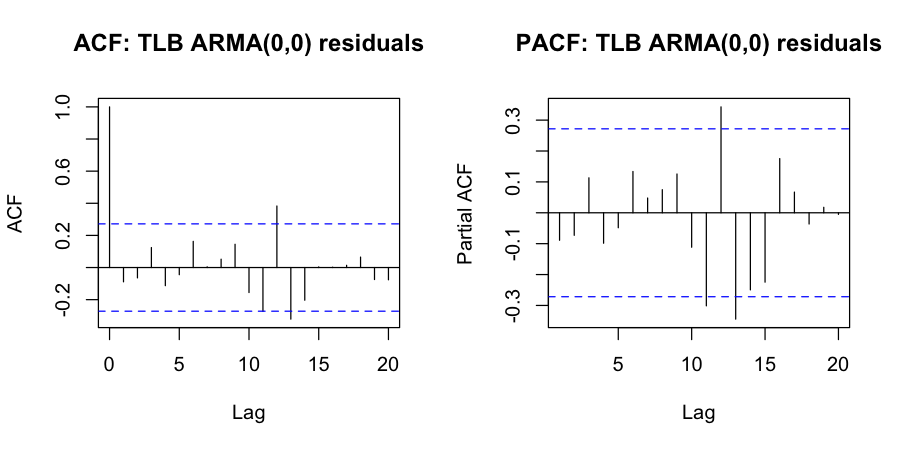
\includegraphics[keepaspectratio,alt={Residual ACF/PACF: TLB ARMA(0,0)}]{plots/13_tlb_arma00_residuals_acf_pacf.png}}
\caption{Residual ACF/PACF: TLB ARMA(0,0)}
\end{figure}

\begin{itemize}
\tightlist
\item
  \textbf{Box--Ljung (lag 10):} p-value = \textbf{0.707} → do not reject
  white-noise residuals at 5\%.
\end{itemize}

\textbf{Conclusion.} ARMA(0,0) is a potential preliminary candidate for
TLB annual changes. In the Final Report we will compare it with at least
one more flexible model (e.g.~AR(1) or ARMA(1,1)) and decide based on
forecast performance on 2013--2024.

\subsubsection{7.2 TFR candidate: AR(1) on annual
changes}\label{tfr-candidate-ar1-on-annual-changes}

\textbf{Model form.} We fit AR(1) on \texttt{diff(TFR\_train)}. In
formula form: \(x_t = c + \phi_1 x_{t-1} + \varepsilon_t\), where
\(x_t\) is the annual change in TFR, \(c\) is a constant, \(\phi_1\) is
the lag-1 effect, and \(\varepsilon_t\) is random shock (white noise).

\textbf{Why this is reasonable.} In the differenced TFR PACF there is a
clear spike at lag 1, while the ACF drops quickly. This is a standard
visual pattern that supports an AR(1) structure.

\begin{itemize}
\tightlist
\item
  \textbf{AIC / BIC (training):} AIC = \textbf{−45.86}, BIC =
  \textbf{−40.01}
\end{itemize}

\begin{figure}
\centering
\pandocbounded{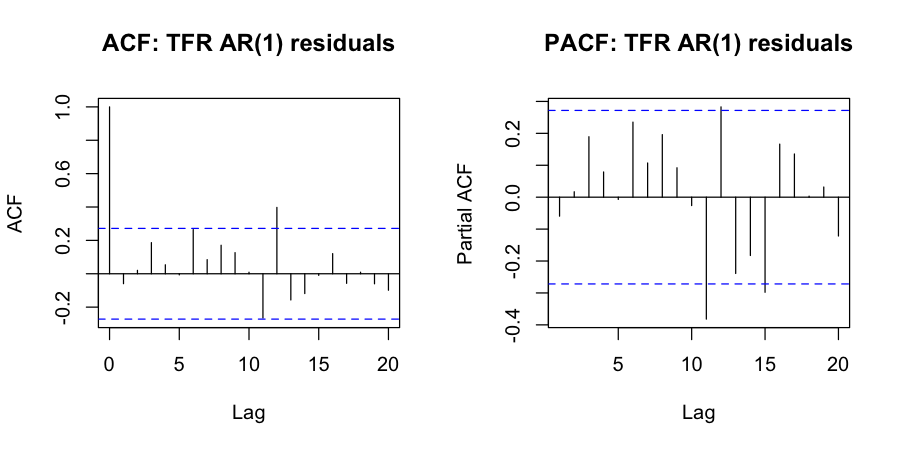
\includegraphics[keepaspectratio,alt={Residual ACF/PACF: TFR AR(1)}]{plots/14_tfr_ar1_residuals_acf_pacf.png}}
\caption{Residual ACF/PACF: TFR AR(1)}
\end{figure}

\begin{itemize}
\tightlist
\item
  \textbf{Box--Ljung (lag 10):} p-value = \textbf{0.439} → do not reject
  white-noise residuals at 5\%.
\end{itemize}

\textbf{Conclusion.} AR(1) on annual changes is a viable preliminary
candidate for TFR. In the Final Report we will still compare it with at
least one alternative ARMA model because fertility has structural breaks
and the ADF result is borderline after differencing.

\begin{center}\rule{0.5\linewidth}{0.5pt}\end{center}

\subsection{8. Model Assessment
Strategy}\label{model-assessment-strategy}

For the Final Report, where we will have at least two models per series
and forecasts for 2013--2024 are needed, the model comparison will use
both in-sample and out-of-sample criteria.

\textbf{In-sample (training fit, 1960--2012):} - AIC and BIC ---
penalise model complexity; lower is better. - Residual diagnostics ---
ACF/PACF of residuals should resemble white noise; Box-Ljung test
p-value should be \textgreater{} 0.05.

\textbf{Out-of-sample (forecast accuracy, 2013--2024):} - Root Mean
Squared Error (RMSE) --- penalises large errors. - Mean Absolute Error
(MAE) --- robust to outliers. - Mean Absolute Percentage Error (MAPE)
--- allows comparison across TLB and TFR scales. - Visual inspection of
forecast vs actual plot --- important for assessing direction and
structural plausibility.

\textbf{Trade-offs.} AIC can prefer more complex models, while BIC
penalises complexity more strongly and often prefers simpler models in
moderate samples like 53 years. A good in-sample fit may still overfit
the historical period (especially with structural breaks). Because of
this, the Final Report will prioritise \textbf{out-of-sample RMSE} on
2013--2024, supported by MAE/MAPE and residual checks.

\begin{center}\rule{0.5\linewidth}{0.5pt}\end{center}

\subsection{9. Summary of EDA Findings and Research Questions
Revisited}\label{summary-of-eda-findings-and-research-questions-revisited}

\textbf{Research question 1 --- Key temporal trends and structural
changes:}\\
Both TLB and TFR show a strong and consistent downward trend from 1960
to 2024. The decline is not smooth --- there are some small shifts
linked to policy events in 1966 and 1987, and an external shock from
COVID-19 in 2020. ADF tests confirm that both level series are
non-stationary, and first differencing achieves stationarity for TLB (p
= 0.039) and near-stationarity for TFR (p = 0.083, borderline).

\textbf{Research question 2 --- Appropriate time series models:}\\
Based on the ACF/PACF structure of the differenced series, ARMA(0,0) is
the potential candidate for TLB annual changes and AR(1) is the
potential candidate for TFR annual changes. Both pass residual
diagnostics at this stage. At least one additional candidate model per
series will be fitted and compared in the Final Report.

\textbf{Research question 3 --- Role of social and policy events:}\\
Policy events are clearly visible in the data. The 1966 family planning
campaign coincides with the sharpest period of decline in both series.
The 1987 pro-natalist policy produced a small and temporary uptick.
COVID-19 produced a dip in TLB around 2020--2021. These features are a
practical limitation for any purely statistical model, and the Final
Report will discuss whether a model that accounts for known break points
performs better than one that does not.

\textbf{Limitations going forward:}\\
The short training sample (n = 53) limits the reliability of
higher-order models and makes it difficult to formally detect structural
breaks. The borderline ADF result for differenced TFR adds uncertainty
to the modelling choice. The test period (2013--2024) includes COVID-19,
which is arguably out-of-sample in a distributional sense and not just a
temporal one.

\begin{center}\rule{0.5\linewidth}{0.5pt}\end{center}

\subsection{10. References}\label{references}

\begin{itemize}
\tightlist
\item
  OBGyn Key n.d., \emph{Singapore's pro-natalist policies: to what
  extent have they worked?}, OBGyn Key, viewed 29 March 2026,
  \url{https://obgynkey.com/singapores-pro-natalist-policies-to-what-extent-have-they-worked/}.
\item
  National Library Board Singapore 2000, \emph{``Have three, or more if
  you can afford it'' is announced}, NLB Singapore, viewed 29 March
  2026,
  \url{https://www.nlb.gov.sg/main/article-detail?cmsuuid=1d106f7e-aca1-4c0e-ac7a-d35d0772707d}.
\item
  United Nations Statistics Division n.d., \emph{Total Fertility Rate:
  Demographics --- Population Change}, UN Statistics Division, viewed 29
  March 2026,
  \url{https://www.un.org/esa/sustdev/natlinfo/indicators/methodology_sheets/demographics/total_fertility_rate.pdf}.
\item
  Hyndman, R.J. \& Athanasopoulos, G. 2021, \emph{Forecasting:
  Principles and Practice}, 3rd edn, OTexts, viewed 29 March 2026,
  \url{https://otexts.com/fpp3/moving-averages.html}.
\item
  Singapore Department of Statistics n.d., \emph{Live Births and
  Fertility Rates}, SingStat, viewed 29 March 2026,
  \url{https://www.singstat.gov.sg/}.
\item
  Urban Redevelopment Authority 2023, \emph{Master Plan}, URA Singapore,
  viewed 29 March 2026,
  \url{https://www.ura.gov.sg/Corporate/Planning/Master-Plan}.
\end{itemize}

\begin{center}\rule{0.5\linewidth}{0.5pt}\end{center}

\subsection{11. Statistical Appendix}\label{statistical-appendix}

\subsubsection{A. Augmented Dickey--Fuller (ADF)
Test}\label{a.-augmented-dickeyfuller-adf-test}

The ADF test assesses whether a time series has a unit root (i.e.~is
non-stationary). The test estimates the regression:

\[
\Delta y_t = \alpha + \beta t + \gamma y_{t-1} + \sum_{j} \delta_j \Delta y_{t-j} + \varepsilon_t
\]

where \(\alpha\) is a constant, \(\beta t\) is an optional linear trend,
\(\gamma\) is the coefficient of interest, and the lagged difference
terms \(\sum_j \delta_j \Delta y_{t-j}\) are included to absorb any
remaining serial correlation in the residuals (this is the ``augmented''
part that distinguishes ADF from the simpler Dickey--Fuller test).

\begin{itemize}
\tightlist
\item
  \textbf{\(H_0\):} \(\gamma = 0\) --- a unit root is present (series is
  non-stationary)\\
\item
  \textbf{\(H_1\):} \(\gamma < 0\) --- no unit root (series is
  stationary)
\end{itemize}

Rejection of \(H_0\) at \(\alpha = 0.05\) (p-value \textless{} 0.05)
provides evidence of stationarity. A failure to reject \(H_0\) suggests
the series has a unit root and may need differencing before modelling.

\subsubsection{B. First Differencing}\label{b.-first-differencing}

If a level series \(y_t\) is non-stationary, the first difference is
defined as:

\[
\Delta y_t = y_t - y_{t-1}
\]

This transformation removes a linear stochastic trend. If one difference
is sufficient to achieve stationarity, the series is said to be
integrated of order one, written \textbf{I(1)}. For TLB and TFR, ADF
evidence supports using one difference.

\subsubsection{C. Autoregressive Model ---
AR(p)}\label{c.-autoregressive-model-arp}

An AR(p) model on a stationary series \(x_t\) (here: the
first-differenced series) is:

\[
x_t = c + \phi_1 x_{t-1} + \phi_2 x_{t-2} + \cdots + \phi_p x_{t-p} + \varepsilon_t
\]

where \(c\) is a constant, \(\phi_1, \ldots, \phi_p\) are autoregressive
coefficients, and \(\varepsilon_t \sim WN(0, \sigma^2)\) is white noise.
The model says the current value depends on its own past \(p\) values.
The order \(p\) is identified from the PACF of the stationary series:
the PACF cuts off sharply after lag \(p\) for a pure AR(p) process.

\subsubsection{D. Moving Average Model ---
MA(q)}\label{d.-moving-average-model-maq}

An MA(q) model on a stationary series \(x_t\) is:

\[
x_t = c + \varepsilon_t + \theta_1 \varepsilon_{t-1} + \theta_2 \varepsilon_{t-2} + \cdots + \theta_q \varepsilon_{t-q}
\]

where \(\theta_1, \ldots, \theta_q\) are moving average coefficients and
\(\varepsilon_t \sim WN(0, \sigma^2)\) is white noise. The model says
the current value depends on current and past \(q\) shocks. The order
\(q\) is identified from the ACF of the stationary series: the ACF cuts
off sharply after lag \(q\) for a pure MA(q) process.

\subsubsection{E. Mixed Model --- ARMA(p,
q)}\label{e.-mixed-model-armap-q}

An ARMA(p, q) model combines both AR and MA components:

\[
x_t = c + \phi_1 x_{t-1} + \cdots + \phi_p x_{t-p} + \varepsilon_t + \theta_1 \varepsilon_{t-1} + \cdots + \theta_q \varepsilon_{t-q}
\]

where all notation is as above. When both ACF and PACF tail off
gradually rather than cutting off sharply, a mixed ARMA model is
suggested. The special case \textbf{ARMA(0,0)} reduces to
\(x_t = c + \varepsilon_t\), meaning the series is pure white noise
around a constant mean --- used here as a baseline model for the
differenced TLB series.

\subsubsection{F. Box--Ljung Portmanteau
Test}\label{f.-boxljung-portmanteau-test}

After fitting a model, the Box--Ljung test checks whether the residual
autocorrelations are jointly zero up to lag \textbf{m}:

\[
Q = n(n+2)\sum_{k=1}^{m} \frac{\hat{r}_k^2}{n-k}
\]

where \(n\) is the number of observations, \(\hat{r}_k\) is the sample
autocorrelation of residuals at lag \(k\), and \(m\) is the chosen
maximum lag (here \(m = 10\)).

\begin{itemize}
\tightlist
\item
  \textbf{\(H_0\):} no autocorrelation in residuals up to lag \(m\)
  (residuals are white noise)\\
\item
  \textbf{\(H_1\):} at least one autocorrelation is non-zero
\end{itemize}

A large p-value (\textgreater{} 0.05) means the residuals are consistent
with white noise, indicating the model has adequately captured the
autocorrelation structure. A small p-value suggests remaining structure
that the model has not captured.

\subsubsection{G. Information Criteria --- AIC and
BIC}\label{g.-information-criteria-aic-and-bic}

Both criteria balance goodness of fit against model complexity:

\[
\mathrm{AIC} = -2\log(L) + 2k
\]

\[
\mathrm{BIC} = -2\log(L) + k\log(n)
\]

where \textbf{L} is the maximised likelihood of the fitted model,
\textbf{k} is the number of estimated parameters, and \textbf{n} is the
number of observations. Lower values of AIC or BIC indicate a better
model. BIC applies a stronger penalty for additional parameters than
AIC, so it tends to favour more parsimonious models, which is important
in small samples like the 53-year training period used here.

\subsubsection{H. Forecast Accuracy Metrics (for Final
Report)}\label{h.-forecast-accuracy-metrics-for-final-report}

When forecasts for 2013--2024 are produced in the Final Report, model
performance will be evaluated using:

\[
\mathrm{RMSE} = \sqrt{\frac{1}{h}\sum_t (y_t - \hat{y}_t)^2}
\]

\[
\mathrm{MAE} = \frac{1}{h}\sum_t \lvert y_t - \hat{y}_t \rvert
\]

\[
\mathrm{MAPE} = \frac{1}{h}\sum_t \frac{\lvert y_t - \hat{y}_t \rvert}{\lvert y_t \rvert}\times 100
\]

where \(h = 12\) is the forecast horizon (2013--2024), \(y_t\) is the
actual value, and \(\hat{y}_t\) is the forecast. RMSE is the primary
criterion as it penalises large errors more heavily, which matters when
forecasting a declining series where large deviations are most costly
for policy use.

\end{document}
